% ShadeWalk LA - CSCI 461 preliminary project report
% Compiles with pdfLaTeX on Overleaf; only standard packages are used.
\documentclass[10pt]{article}   % 10pt is the conference-paper norm and keeps us near 10 pages

\usepackage[margin=1in]{geometry}
\usepackage{graphicx}
\usepackage{booktabs}
\usepackage{amsmath}
\usepackage{amssymb}
\usepackage{caption}
\usepackage{subcaption}
\usepackage{float}
\usepackage{url}
% numeric citations like the example report: \citep -> [6], \citet -> Hoffman et al. [6].
% "square" is needed for [6] rather than (6); sort&compress turns [3,1,2] into [1-3].
\usepackage[numbers,square,sort&compress]{natbib}
\usepackage[colorlinks=true,allcolors=blue]{hyperref}
\usepackage{siunitx}
\sisetup{detect-weight=true}

\graphicspath{{../figures/}}

\title{\textbf{ShadeWalk LA: Recommending Cooler Pedestrian Routes\\
from Satellite Land Surface Temperature}}

\author{
  \begin{tabular}{c@{\hspace{4em}}c}
    \textbf{Ethan Chiu}     & \textbf{Junseo Lee} \\
    \texttt{chiuetha@usc.edu} & \texttt{junseole@usc.edu}    \\[1.5em]
    \textbf{Nathan Nguyen}     & \textbf{Sinchana Nama}    \\
    \texttt{nathann3@usc.edu}   & \texttt{snama@usc.edu}
  \end{tabular}
}
\date{}

\begin{document}
\maketitle

\begin{abstract}
Extreme heat is the deadliest weather hazard in the United States, and in a car-centric city
such as Los Angeles those most exposed are the people who walk --- yet every navigation app
optimises distance alone. We ask whether free satellite and land-cover data suffice to
recommend a measurably cooler walking route. Fusing ECOSTRESS land surface temperature (LST)
with NLCD canopy and impervious rasters, our central finding is negative and instructive:
predicting \emph{absolute} LST under a random or purely spatial split reports $R^2 = 0.87$,
but the same models fall to $R^2 \approx 0$ once held-out \emph{dates} are introduced ---
almost all the apparent skill was the model recalling how hot each overpass was. Re-posing
the task as the \emph{within-scene anomaly} $\Delta$LST, which is what a router actually
compares, gives a model that is modest ($R^2 = 0.35 \pm 0.04$ under a joint
spatial-and-temporal split) but stable, and in which neighbourhood tree canopy is the only
variable whose removal costs more than $0.02$ of $R^2$. Judged on what routing needs ---
ordering, not calibration --- it picks the cooler of two locations in an unseen scene
\SI{72.7}{\percent} of the time. Over 60 origin--destination pairs sampled evenly across
low-, medium- and high-canopy neighbourhoods, however, only \SI{14}{\percent} admit an
alternative at least \SI{1}{\celsius} cooler, and the system reroutes just
\SI{1.7}{\percent} of trips -- far below the \SI{70}{\percent} reported for a
building-shadow-aware system on a single university campus. We built and tested a
building-shadow feature of our own to probe that gap directly; it made the temperature
model slightly worse, not better, which we read as evidence about what \SI{70}{\metre}
satellite temperature can resolve rather than about whether Los Angeles has shade to offer.
\end{abstract}

%====================================================================
\section{Introduction}
\label{sec:intro}

\subsection{Motivation}

\subsubsection{Urban heat and pedestrians}
Heat kills more people in the United States each year than hurricanes, floods and tornadoes
combined, and the hazard is not evenly distributed within a city. Dense, paved, treeless
blocks store solar energy and release it slowly --- the urban heat island effect --- so
surface temperatures inside one city can differ by more than \SI{15}{\celsius} at the same
instant. This is not accidental: across 108 US urban areas \citet{hoffman2020redlining}
found formerly redlined neighbourhoods on average \SI{2.6}{\celsius} hotter, and up to
\SI{7}{\celsius} hotter in individual cities, so the hottest streets fall disproportionately
in lower-income neighbourhoods whose residents are least likely to own a car.

Pedestrians bear this most directly. Someone walking \SI{2}{\kilo\metre} to a bus stop at
2~pm in July controls nothing about the surfaces they cross except the route --- and that
choice is currently made for them by software optimising distance alone.

\subsubsection{Why this is a sustainable development problem}
Three UN Sustainable Development Goals name this problem: \textbf{Goal~3} (good health ---
heat stress and heat stroke are direct, preventable harms), \textbf{Goal~11} (sustainable
cities --- walkability collapses when walking is unpleasant or dangerous, pushing people
back into cars), and \textbf{Goal~13} (climate action --- heat waves are intensifying, so
adaptation is needed alongside mitigation). We address Goals~3 and~11: given that the heat
already exists, we try to help people move through the city with less exposure to it.

\subsection{Problem statement}
Given an origin $s$ and a destination $d$ within Los Angeles, and the current local time $t$,
recommend a walking route $r$ from a set of candidate routes $R(s,d)$ that trades off
predicted thermal exposure against detour length. Concretely, for each candidate route we
predict a surface temperature profile along the path from land cover, terrain and time of
day; we discard candidates longer than $\tau$ times the shortest route; and among the
remainder we minimise a weighted combination of mean predicted temperature, lack of tree
canopy, and distance. The recommendation falls back to the shortest route unless the
predicted cooling exceeds a minimum threshold, so that the system never trades a meaningful
detour for a negligible thermal gain.

\subsection{High-level outline of goals and approaches}
We combine data from two sources --- ECOSTRESS thermal imagery and the National Land Cover
Database --- and derive several further variables from them. We clean the fused table with a
sequence of quality filters whose effect is reported stage by stage. We then explore the data
with histograms, scatter plots, a correlation matrix and a variance decomposition; that last
diagnostic is what drove the central design decision of this report. We establish a linear
regression baseline and compare it against regularised linear, decision tree, random forest
and histogram gradient boosting models, under two prediction targets and four
cross-validation designs. Finally we evaluate the end-to-end router against a shortest-path
baseline on a fixed set of origin--destination pairs.

%====================================================================
\section{Related Work}
\label{sec:related}

\paragraph{Satellite estimation of urban surface temperature.}
Urban heat islands are usually mapped from Landsat~8 TIRS (\SI{100}{\metre},
\SI{16}{\day} revisit). ECOSTRESS \citep{fisher2020ecostress} suits us better: its
non-sun-synchronous orbit samples different times of day, which Landsat --- always crossing
near 10:30~am local --- cannot. Its Level-2 LST product validates against ground stations at
RMSE \SI{1.07}{\kelvin} \citep{hulley2021validation}, well inside our tolerance. Prior work
reports negative association between vegetation and LST and positive association with
impervious fraction; our correlations (Section~\ref{sec:eda}) reproduce this.

\paragraph{Thermally aware routing.}
\citet{buo2026coolroutes} build \emph{Cool Routes} for the Arizona State University campus
in Tempe: mean radiant temperature (MRT) forecast at \SI{1}{\metre} with the SOLWEIG
radiation model from building and tree data plus hourly meteorology, used as edge impedance
in Dijkstra's algorithm. Over 500 origin--destination pairs on 12 clear days they reroute in
more than \SI{70}{\percent} of cases, cutting average MRT by up to \SI{3.8}{\celsius} for
detours under \SI{3}{\percent}, validated against the MaRTy mobile platform ($d = 0.73$).
\citet{wolf2025coolwalks} instead analyse the network: from building footprints and heights
--- \emph{building} shade only, no trees --- they define a CoolWalkability metric for
Manhattan, Barcelona and Valencia, and show analytically that a regular grid of constant
building height offers a shade-seeking pedestrian \emph{no} benefit over the shortest path,
with shade opportunity otherwise forming spatial clusters.

Both are more physically faithful than ours, and both need inputs --- building heights, tree
inventories, hourly meteorology, a radiation model --- available for few places; Cool Routes
covers one campus. We sit at the other end of the cost spectrum: two public global rasters
and a free routing API, no 3D city model. This also sets expectations, since MRT at
\SI{1}{\metre} resolves the shadow on a specific sidewalk and \SI{70}{\metre} LST cannot
(Section~\ref{sec:routes}).

\paragraph{Evaluation of spatially structured models.}
\citet{roberts2017crossvalidation} argue for block cross-validation wherever a dependence
structure exists, and \citet{ploton2020spatial} show that ignoring spatial autocorrelation
moved the reported $R^2$ of a continental biomass model between $0.14$ and $0.53$ on
validation design alone. Our results (Section~\ref{sec:results}) extend the warning to a
second axis: for \emph{repeat} satellite imagery the temporal dimension leaks at least as
badly, since spatial blocking alone left our $R^2$ at $0.865$ while holding out dates
revealed it to be near zero. Spatial blocking is necessary but not sufficient.

To our knowledge no prior work recommends pedestrian routes in Los Angeles from ECOSTRESS
LST, and we have not seen the absolute-versus-anomaly target distinction made explicit in
this literature, although in our setting it changes the reported $R^2$ by almost a full unit.

%====================================================================
\section{Data}
\label{sec:data}

We draw on two primary sources and derive five further variables from them. All data are
public and free; no commercial API was used in the modelling pipeline.

\subsection{ECOSTRESS land surface temperature}
ECOSTRESS (ECOsystem Spaceborne Thermal Radiometer Experiment on Space Station)
\citep{fisher2020ecostress} produces the \texttt{ECO\_L2T\_LSTE} v002 product
\citep{hook2022lste}: gridded land surface temperature at \SI{70}{\metre} resolution,
delivered as one GeoTIFF per layer per granule. We downloaded all granules
intersecting the Los Angeles bounding box
($\text{lon} \in [-118.63, -117.56]$, $\text{lat} \in [33.88, 34.40]$) for June--August 2026:
\textbf{131 granules} across four MGRS tiles (11SLT, 11SLU, 11SMT, 11SMU), each with eight
layers.

We use five of the eight layers: \texttt{LST} (float32 Kelvin, converted to \si{\celsius});
\texttt{QC}, keeping only pixels whose two lowest bits are 0 (best) or 1 (nominal);
\texttt{cloud} and \texttt{water}, both of which must be zero; and \texttt{LST\_err}, the
per-pixel retrieval uncertainty, since thin cloud escaping the cloud mask shows up here as
elevated error (we discard $\texttt{LST\_err} > \SI{2.0}{\kelvin}$). A sixth layer,
\texttt{height}, carries terrain elevation, which we exploit to obtain a DEM with no extra
download (Section~\ref{sec:derived}).

Filename timestamps are UTC; we convert to America/Los\_Angeles and keep only granules whose
local overpass falls in $[8, 19)$ hours, since the night-time regime is governed by different
physics that our application does not model.

\subsection{National Land Cover Database}
NLCD \citep{dewitz2023nlcd} provides \SI{30}{\metre} rasters for the contiguous United
States. We use two products: \textbf{Tree Canopy Cover} and \textbf{Percent Developed
Imperviousness}, both expressed as \SIrange{0}{100}{\percent}. The imperviousness raster ships as a single \SI{997}{\mega\byte}
CONUS file; we clip it once to the Los Angeles box with a \ang{0.05} margin, reducing it to
\SI{4.3}{\mega\byte} and leaving the original untouched. Both rasters are in CONUS Albers
projection and are reprojected on the fly when sampled at a longitude/latitude pair.

\subsection{Derived variables}
\label{sec:derived}
Five further variables are computed from the two sources above:

\texttt{canopy\_100m} and \texttt{impervious\_100m} are the mean of the corresponding raster
over a square window of radius \SI{100}{\metre} ($7 \times 7$ pixels), nodata excluded from
both numerator and denominator. The motivation is physical --- what cools a walking person is
the tree cover of the surrounding block, not the single \SI{30}{\metre} cell underfoot ---
and it matters a great deal (Table~\ref{tab:features}). \texttt{elevation\_m} is a mosaic of
the ECOSTRESS \texttt{height} layers over the four tiles; terrain does not change between
overpasses, so a few granules per tile suffice and the per-pixel maximum fills nodata gaps.
\texttt{dist\_coast\_km} is distance to the Pacific: NLCD covers land only, so the large
connected nodata region west of the city \emph{is} the ocean, and we distance-transform from
its largest connected component --- again avoiding an external download. \texttt{hour} is the
local overpass time as a decimal hour.

\subsection{Data fusion and cleaning}
\label{sec:fusion}
Table~\ref{tab:funnel} reports how many granules and pixels survive each stage of cleaning.
Two filters were added after an initial pass revealed residual cloud contamination: the
minimum temperature in the first version of our table was \SI{-9.99}{\celsius} and the coldest
scene averaged \SI{4.3}{\celsius}, both physically implausible for Los Angeles in summer. The
two additions are
(i) a \emph{granule-level} rule discarding any scene in which fewer than \SI{30}{\percent} of
the pixels inside the Los Angeles box survive masking, and
(ii) a \emph{within-scene} robust outlier cut removing pixels more than $4 \times$ the median
absolute deviation from the scene median. After these, the coldest pixel is
\SI{9.59}{\celsius} and the coldest scene mean \SI{12.1}{\celsius}.

The cost is real --- 45 of 107 daytime granules are discarded, taking us from 23 dates to 18
--- but the benefit is measurable: the correlation between neighbourhood canopy and the
within-scene temperature anomaly strengthened from $-0.326$ to $-0.487$, i.e.\ removing cloud
sharpened precisely the signal we are trying to learn.

\begin{table}[H]
\centering
\caption{Data funnel. Pixel counts are summed over all daytime granules.}
\label{tab:funnel}
\small
\begin{tabular}{lrl}
\toprule
Stage & Count & Criterion \\
\midrule
Granules downloaded                  & 131 & LA bounding box, Jun--Aug 2026 \\
Granules in daytime window           & 107 & 8--19\,h local \\
Granules after valid-fraction filter & 62  & $\geq \SI{30}{\percent}$ of LA-box pixels valid \\
Granules used                        & 62  & $\geq 200$ sampled pixels \\
\midrule
Pixels inside LA box        & 37{,}054{,}611 & before any masking \\
After LST range check       & 23{,}367{,}415 & $-10$ to \SI{75}{\celsius} \\
After cloud mask            & 23{,}367{,}415 & \texttt{cloud} $= 0$ \\
After water mask            & 22{,}577{,}664 & \texttt{water} $= 0$ \\
After QC mask               & 22{,}577{,}664 & QC bits 0--1 $\in \{0,1\}$ \\
After \texttt{LST\_err} cut & 20{,}119{,}183 & $\leq \SI{2.0}{\kelvin}$ \\
After robust MAD cut        & 20{,}024{,}828 & $4 \times$ MAD from scene median \\
\midrule
Rows sampled                   & 248{,}000 & $\leq 4000$ per granule \\
Rows after land-cover join     & 243{,}468 & all features present \\
\bottomrule
\end{tabular}
\end{table}

Random sampling of up to 4000 pixels per granule keeps the table at a workable size; the
final fused dataset has \textbf{243{,}468 rows} over \textbf{62 granules} and
\textbf{18 distinct dates}.

\subsection{Feature set}
Table~\ref{tab:features} lists the variables used for regression, following the format of
prior preliminary reports in this course. We report the coefficient of variation
(standard deviation divided by mean) as a measure of relative spread, and additionally the
correlation of each variable with the within-scene temperature anomaly, since that is the
target we will argue for in Section~\ref{sec:target}.

\begin{table}[H]
\centering
\caption{Features used for regression. CV is the coefficient of variation; the last column
is the Pearson correlation with $\Delta\text{LST}$.}
\label{tab:features}
\small
\begin{tabular}{llllrrr}
\toprule
Feature & Source & Type & Derived? & Mean & CV & $r$ with $\Delta$LST \\
\midrule
\multicolumn{7}{l}{\emph{Shipped model (six variables)}} \\
\texttt{canopy\_100m}     & NLCD      & float & Yes & 15.02   & 0.790  & $-0.487$ \\
\texttt{impervious\_100m} & NLCD      & float & Yes & 16.24   & 1.603  & $+0.332$ \\
\texttt{elevation\_m}     & ECOSTRESS & float & Yes & 955.12  & 0.724  & $-0.167$ \\
\texttt{lat}              & ECOSTRESS & float & No  & 34.24   & 0.004  & $-0.058$ \\
\texttt{lon}              & ECOSTRESS & float & No  & $-118.05$ & $-0.003$ & $+0.004$ \\
\texttt{hour}             & ECOSTRESS & float & Yes & 13.25   & 0.242  & $+0.000$ \\
\midrule
\multicolumn{7}{l}{\emph{Computed but dropped after ablation (Section~\ref{sec:robust-results})}} \\
\texttt{canopy\_pct}      & NLCD      & float & No  & 15.03   & 0.988  & $-0.401$ \\
\texttt{impervious\_pct}  & NLCD      & float & No  & 16.25   & 1.668  & $+0.322$ \\
\texttt{dist\_coast\_km}  & NLCD      & float & Yes & 57.43   & 0.350  & $+0.004$ \\
\bottomrule
\end{tabular}
\end{table}

Two observations from this table shaped the rest of the work. First, the
\emph{neighbourhood-averaged} canopy variable is a markedly stronger correlate of local
temperature anomaly ($-0.487$) than the raw pixel value ($-0.401$), confirming the physical
intuition behind the derived feature; the ablation later shows the raw pixel value adds
nothing once the neighbourhood mean is present. Second, \texttt{hour} and
\texttt{dist\_coast\_km} have essentially zero linear correlation with the anomaly, yet both
receive substantial impurity-based importance from tree models --- a discrepancy we return to
in Sections~\ref{sec:importance} and~\ref{sec:robust-results}, and which ultimately removed
\texttt{dist\_coast\_km} from the model.

\subsection{Exploratory data analysis}
\label{sec:eda}

\paragraph{Distributions and scene-level structure.}
Absolute LST is broad and multi-modal, reflecting scenes recorded at different times and
under different synoptic conditions; granule means span roughly \SIrange{12}{48}{\celsius}
across our 62 scenes. The within-scene anomaly, by contrast, is unimodal and roughly
symmetric with a standard deviation of about \SI{4.4}{\celsius}. That contrast is the source
of the problem described next.

\paragraph{Variance decomposition --- the key diagnostic.}
Decomposing the total variance of the LST column into a between-scene component and a
within-scene component (Figure~\ref{fig:variance}) shows that \textbf{\SI{75}{\percent} of
the variance is between scenes} --- i.e.\ it is explained by \emph{which day the satellite
flew over}, not by where in the city the pixel is. Only \SI{25}{\percent} is the spatial
structure within a single snapshot.

This matters because our application never compares across scenes. A pedestrian choosing
between two routes at 2~pm on a given day is asking a purely within-scene question. A model
that captures the between-scene component beautifully and the within-scene component poorly
would report excellent aggregate metrics while being useless for routing.

\begin{figure}[H]
\centering
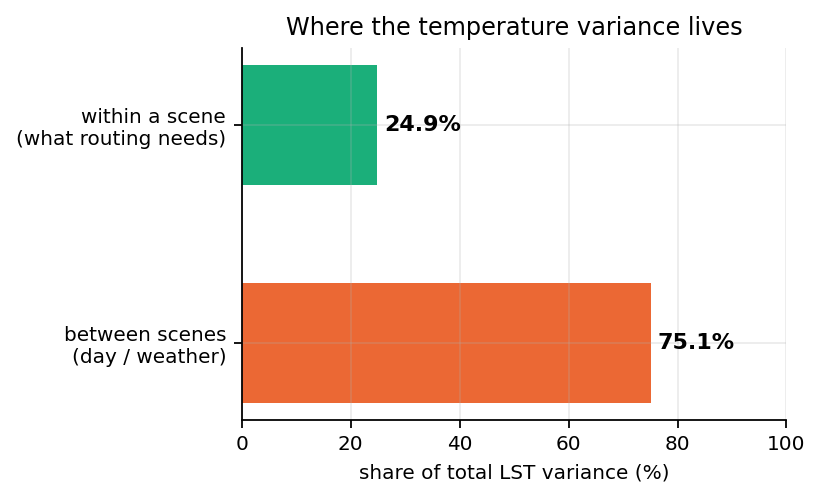
\includegraphics[width=0.62\textwidth]{variance_decomposition.png}
\caption{Variance decomposition of land surface temperature. Three quarters of the variance
is between satellite overpasses; only the remaining quarter is the spatial signal that route
recommendation actually depends on.}
\label{fig:variance}
\end{figure}

\paragraph{Land cover versus temperature.}
Figure~\ref{fig:landcover} plots canopy and impervious fraction against absolute LST and
against the anomaly. Against absolute LST the relationship is visually weak, swamped by
scene-to-scene variation; against the anomaly a clean monotone relationship emerges, with
zero to \SI{60}{\percent} neighbourhood canopy worth roughly \SI{8}{\celsius} of local
cooling.

\begin{figure}[H]
\centering
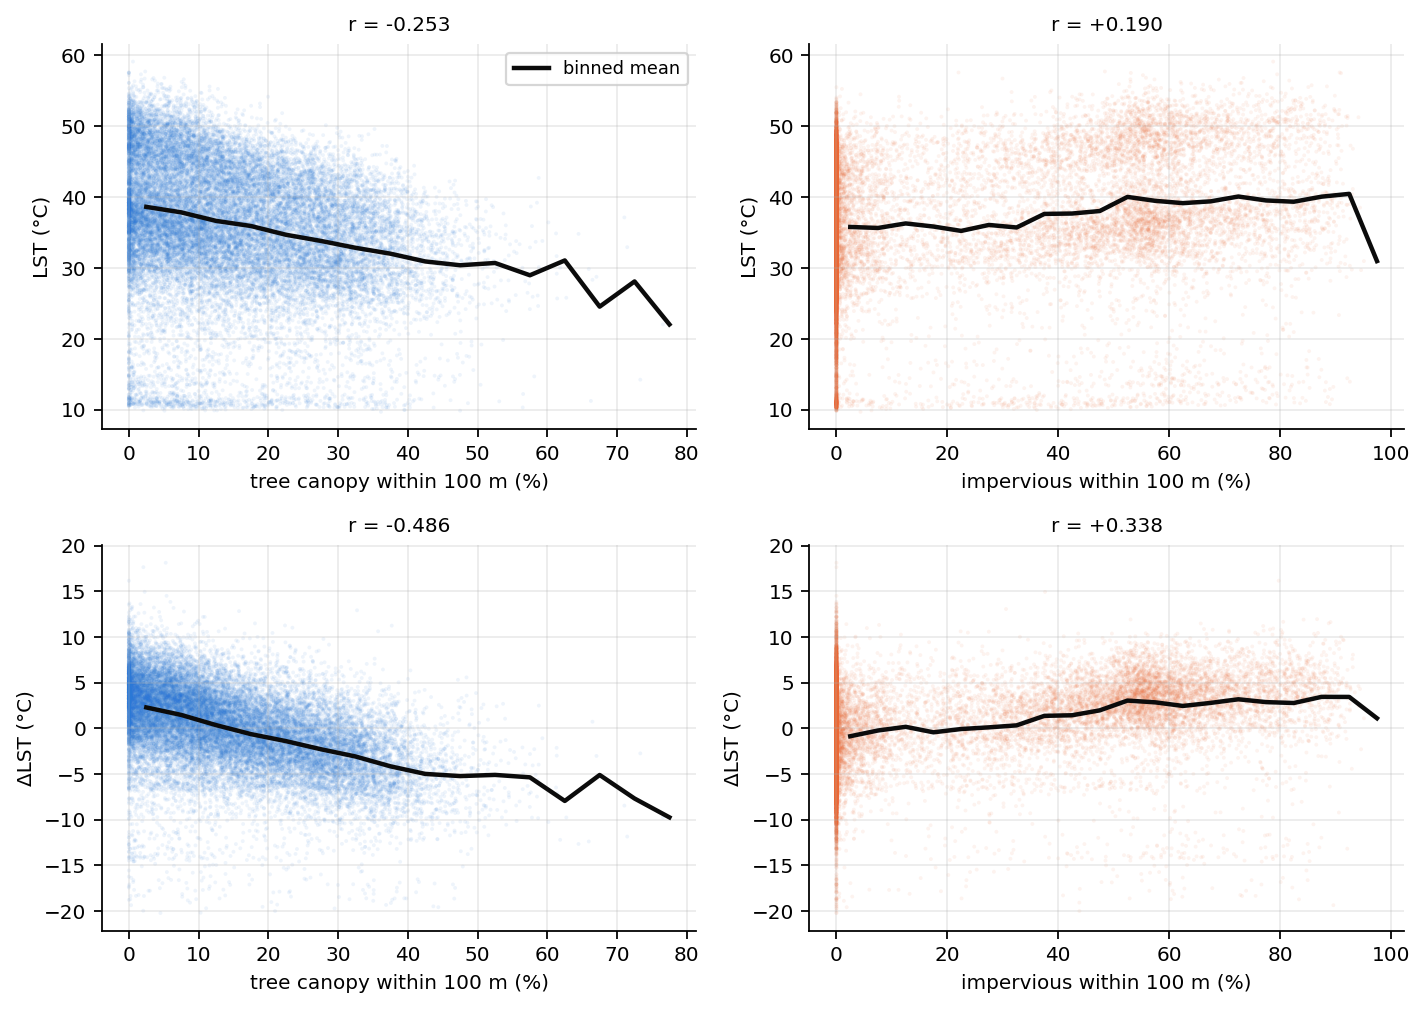
\includegraphics[width=0.95\textwidth]{landcover_vs_lst.png}
\caption{Neighbourhood canopy and impervious fraction against absolute LST (top) and against
the within-scene anomaly (bottom). Black lines are binned means.}
\label{fig:landcover}
\end{figure}

\paragraph{Correlation structure.}
Figure~\ref{fig:corr} gives the correlation matrix. Each land-cover variable is strongly
correlated with its neighbourhood-averaged counterpart, as expected since they measure the
same quantity at two scales --- redundancy the ablation in Section~\ref{sec:robust-results}
later exploits. Raw scales differ by orders of magnitude, so features are standardised for
the linear models.

\begin{figure}[H]
\centering
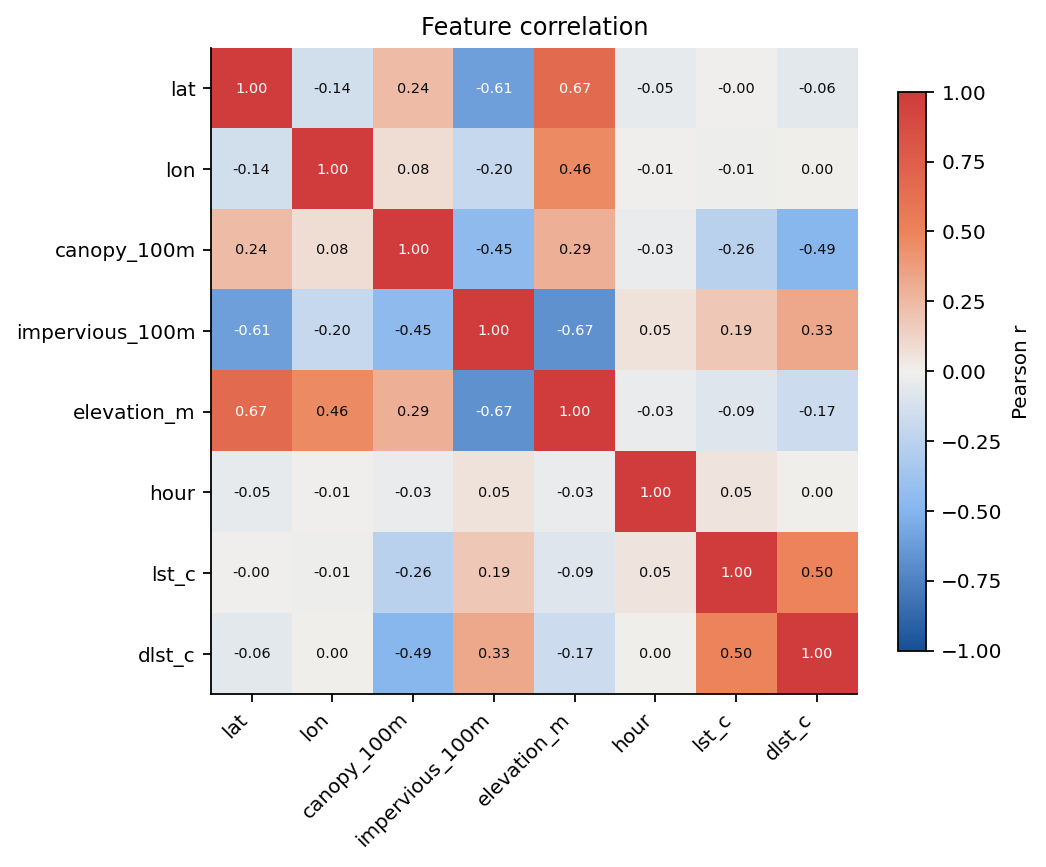
\includegraphics[width=0.56\textwidth]{correlation_matrix.png}
\caption{Feature correlation matrix.}
\label{fig:corr}
\end{figure}

%====================================================================
\section{Task, Approach and First Empirical Results}
\label{sec:task}

This section states the learning task, the approaches compared, and the results obtained so
far. Section~\ref{sec:task-def} defines the task and the two targets;
Sections~\ref{sec:splits}--\ref{sec:routing-approach} give the approach; the remainder
reports results.

\subsection{Task definition and two prediction targets}
\label{sec:task-def}

\label{sec:target}
Motivated by Figure~\ref{fig:variance}, we train and evaluate every model under two targets:
\begin{align}
  \text{\texttt{lst}:}  \quad & y_i = \text{LST}_i \\
  \text{\texttt{dlst}:} \quad & y_i = \Delta\text{LST}_i = \text{LST}_i - \frac{1}{|G(i)|}\sum_{j \in G(i)} \text{LST}_j
\end{align}
where $G(i)$ is the set of pixels belonging to the same granule as pixel $i$. The second
target removes the scene-level offset, leaving exactly the spatial signal that routing uses.
Because route comparison is relative --- we only ever ask which of several simultaneous paths
is cooler --- predicting the anomaly loses no information the application needs.

\subsection{Approach: four evaluation designs}
\label{sec:splits}
Models are scored under four three-fold designs. \textbf{random} is plain $K$-fold, the naive
reference point and what the comparable prior report in this course used.
\textbf{spatial} is \texttt{GroupKFold} on \ang{0.05} ($\approx$\SI{5}{\kilo\metre}) blocks,
so nearby pixels cannot straddle the split. \textbf{temporal} is \texttt{GroupKFold} on
calendar date. \textbf{spatial\,+\,temporal} is the strict design: blocks and dates are each
partitioned into folds, a test row must lie in an unseen block \emph{and} fall on an unseen
date, a training row in neither, and rows meeting only one condition are dropped from that
fold. The last corresponds to real deployment --- the system is asked about streets it has
not seen, on a day it has not seen.

\subsection{Approach: models}
We compare five regressors: ordinary least squares (baseline), ridge, a decision tree, a
random forest \citep{breiman2001randomforests}, and histogram-based gradient boosting, whose
binned construction follows \citet{ke2017lightgbm}; all are scikit-learn implementations
\citep{pedregosa2011scikitlearn}. Ensemble hyperparameters come from a small grid searched
inside the training folds of the strict split (forest: \texttt{max\_depth}
$\in \{10, 20, \text{None}\}$, \texttt{min\_samples\_leaf} $\in \{5, 50\}$; boosting:
\texttt{learning\_rate} $\in \{0.05, 0.1\}$, \texttt{max\_depth} $\in \{4, 8\}$), reused
across the other splits --- a fully nested search over every cell would multiply runtime, and
Section~\ref{sec:robust-results} verifies the shortcut did not change the ranking. The grid
runs on a granule-stratified subsample of 60{,}000 rows; the shipped model uses the full
table. We report RMSE, MAE and $R^2$ as mean $\pm$ sd over folds.

\subsection{Approach: robustness checks}
\label{sec:robustness}
Three folds over 18 dates is too coarse to quote a single number from, and the tuning
shortcut is a potential source of optimism, so we add four checks.
\textbf{Leave-one-date-out} trains on 17 dates and tests on the 18th, once per date, giving
18 estimates summarised by a 10{,}000-resample bootstrap interval. \textbf{Nested
cross-validation} re-runs the hyper-parameter search inside each outer training fold, so the
reported score never sees a fold used for tuning. \textbf{Leave-one-feature-out ablation}
drops each feature in turn --- Section~\ref{sec:importance} singles out \texttt{hour} as a
suspected scene identifier, and applying the same test to \emph{every} variable avoids
suspecting only the feature we happened to notice. \textbf{Within-scene ranking} measures,
per held-out scene, the Spearman correlation between predicted and observed anomaly and the
\emph{pairwise accuracy} --- given two random pixels in one scene, how often the cooler is
identified. Route scoring needs ordering, not calibration, so this is the quantity that
corresponds to fitness for purpose and $R^2$ is not.

\subsection{Approach: route recommendation}
\label{sec:routing-approach}
Candidate routes come from the OpenRouteService \citep{ors2026} foot-walking profile over
the OpenStreetMap pedestrian network \citep{osm}, using both its native alternative-routes
feature and extra queries through perpendicular offset waypoints, since short urban trips
often admit only one native alternative. Each candidate is resampled at \SI{50}{\metre} and
scored by the model; candidates longer than $\tau = 1.3\times$ the shortest are discarded.
Among the rest we minimise
\begin{equation}
  \text{score}(r) = w_h \, \tilde{H}(r) + w_s \, \bigl(1 - \tilde{S}(r)\bigr) + w_d \, \tilde{D}(r)
\end{equation}
where $\tilde{H}$, $\tilde{S}$, $\tilde{D}$ are mean predicted temperature, mean canopy
fraction and length, each min--max normalised across the candidate set, with
$(w_h, w_s, w_d) = (0.4, 0.3, 0.3)$ by default. The recommendation reverts to the shortest
route unless predicted mean cooling exceeds \SI{1.0}{\celsius}, so a detour is proposed only
when it buys something.

%====================================================================
\subsection{Results: target and split both change the answer}
\label{sec:results}

Table~\ref{tab:models} is the central result of this report. Reading it by rows gives the
usual model comparison; reading it by columns gives something more interesting.

\begin{table}[H]
\centering
\caption{$R^2$ (mean over 3 folds) for every combination of target, split and model. The
upper block predicts absolute LST; the lower block predicts the within-scene anomaly. Best
model per column in each block is shown in bold.}
\label{tab:models}
\small
\begin{tabular}{llrrrr}
\toprule
Target & Model & random & spatial & temporal & spatial\,+\,temporal \\
\midrule
\texttt{lst} & Linear               & 0.104 & 0.102 & $-0.197$ & $-0.075$ \\
             & Ridge                & 0.104 & 0.102 & $-0.197$ & $-0.075$ \\
             & Decision tree        & 0.866 & 0.848 & $-0.429$ & $-0.495$ \\
             & Random forest        & 0.847 & 0.836 & $-0.231$ & $\mathbf{0.045}$ \\
             & Gradient boosting    & \textbf{0.875} & \textbf{0.865} & $-0.271$ & $-0.102$ \\
\midrule
\texttt{dlst} & Linear              & 0.317 & 0.314 & 0.305 & 0.300 \\
              & Ridge               & 0.317 & 0.314 & 0.305 & 0.300 \\
              & Decision tree       & 0.508 & 0.437 & 0.218 & 0.199 \\
              & Random forest       & 0.516 & 0.472 & \textbf{0.366} & \textbf{0.354} \\
              & Gradient boosting   & \textbf{0.565} & \textbf{0.522} & 0.300 & 0.302 \\
\bottomrule
\end{tabular}
\end{table}

Three findings follow.

\paragraph{Finding 1: the headline $R^2$ of the naive setup is an artefact.}
Predicting absolute LST on a random split gives $R^2 = 0.875$, and blocking in space barely
changes it ($0.865$) --- but holding out \emph{dates} collapses it to $-0.271$, with the best
strict-split model reaching only $0.045$ and three of five negative. A negative $R^2$ means
the model does worse than predicting the mean. The apparent skill was the model inferring
from latitude, longitude and hour \emph{which granule} a pixel came from, then recalling that
granule's temperature level. Spatial blocking --- the standard remedy --- does not catch
this, because the leak runs along the time axis.

Our own earlier pipeline, before this analysis, reported $R^2 = 0.891$ under exactly the
naive configuration. We report it here as a cautionary data point rather than as a result.
The magnitude of the gap is comparable to what \citet{ploton2020spatial} documented for
spatial leakage in ecological mapping, which supports their broader argument
\citep{roberts2017crossvalidation} that the validation design, not the model, is often what
determines a headline number.

\paragraph{Finding 2: the anomaly target is stable.}
Under \texttt{dlst} every model degrades gracefully from random ($0.565$) to strict
($0.354$) rather than falling off a cliff (Figure~\ref{fig:modelcomp}). The strict-split
numbers are modest, but they are numbers we believe.

\begin{figure}[H]
\centering
\begin{subfigure}{0.49\textwidth}
  \centering
  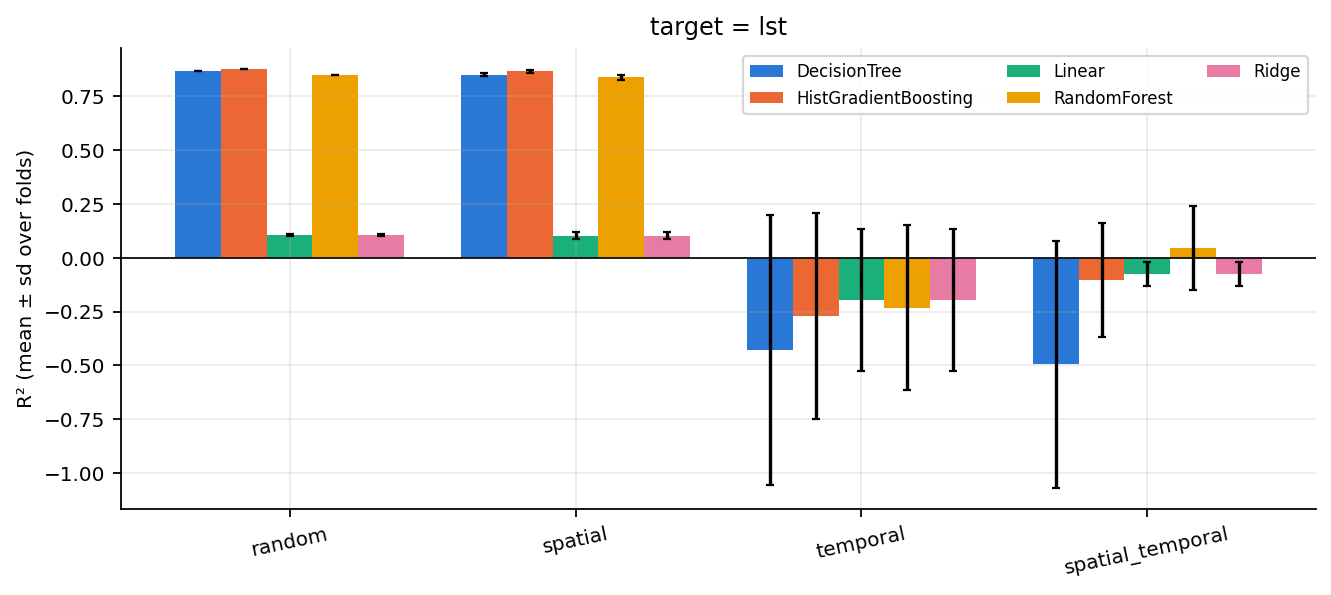
\includegraphics[width=\textwidth]{model_comparison_lst.png}
  \caption{Target = absolute LST.}
\end{subfigure}\hfill
\begin{subfigure}{0.49\textwidth}
  \centering
  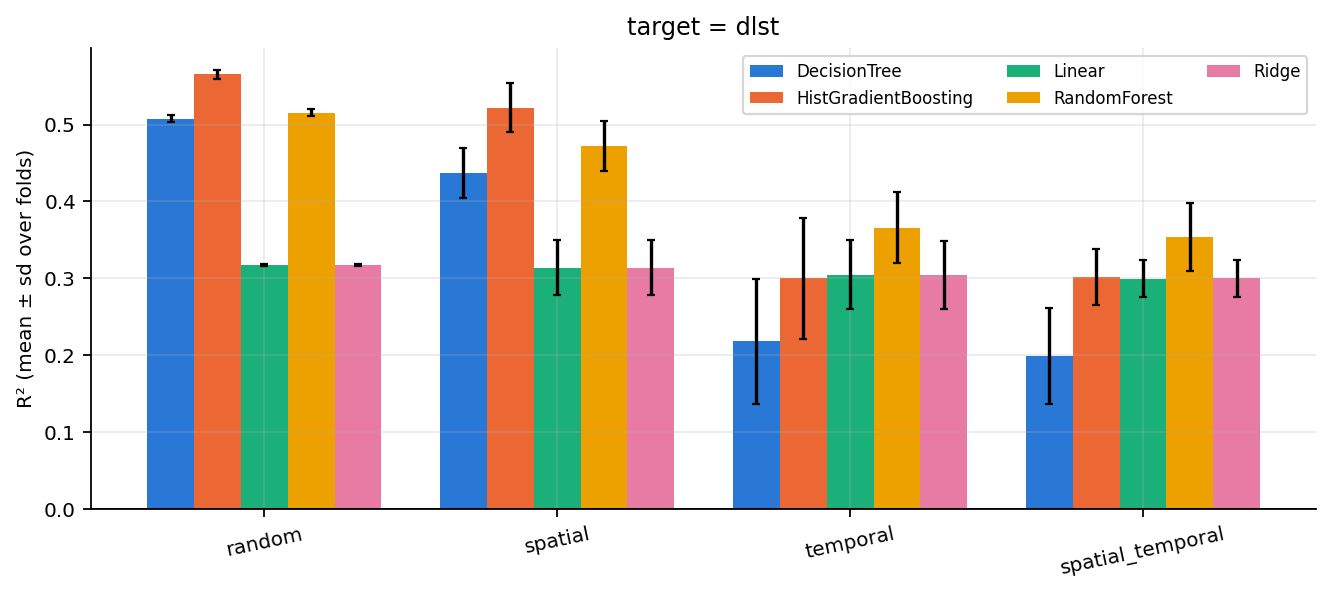
\includegraphics[width=\textwidth]{model_comparison_dlst.png}
  \caption{Target = within-scene anomaly.}
\end{subfigure}
\caption{$R^2$ by split and model. With the absolute target, performance collapses as soon as
dates are held out; with the anomaly target it degrades gradually.}
\label{fig:modelcomp}
\end{figure}

\paragraph{Finding 3: the model ranking depends on the split.}
Gradient boosting wins under random and spatial splits; the random forest wins once dates
are held out. The gap to the linear baseline also narrows sharply --- under the strict split
OLS ($0.300$) is within $0.06$ of the random forest ($0.354$), against $0.25$ under a random
split --- so the extra capacity of tree ensembles is largely spent on structure that does
not transfer.

In absolute terms the best \texttt{dlst} model under the strict split reaches
RMSE \SI{3.56}{\celsius} and MAE \SI{2.61}{\celsius} on the \num{60000}-row subsample used
for this model-comparison grid; the best \texttt{lst} model under the same split reaches
RMSE \SI{8.04}{\celsius}, more than twice as large. The shipped model in
Section~\ref{sec:routes}, refit on the full \num{243468}-row dataset, lands close but not
identical (RMSE \SI{3.62}{\celsius}) --- the gap is the subsample, not a different split or
feature set.

On a held-out strict fold the shipped model captures the broad spatial pattern but
systematically under-predicts the extremes, a regression to the mean typical of averaged
ensembles.

\subsection{Results: feature importance, impurity versus permutation}
\label{sec:importance}
\texttt{canopy\_100m} dominates on both measures (permutation importance $0.348$, next
largest $0.175$), which is the physically expected result and a reassuring one: the variable
the router can act on is the variable that matters.

The instructive disagreement is \texttt{hour}. Impurity importance ranks it second
($0.181$); permutation importance on the held-out fold ranks it \emph{last of six}
($0.014$). The explanation is in the data --- our 62 granules fall on only 18 dates, each
with a near-unique overpass time, so \texttt{hour} is a quasi-identifier for the scene. A
tree splits on it eagerly in training; on an unseen date that identifier is meaningless.
This is Finding~1 again, seen from the feature side, and the ablation in
Section~\ref{sec:robust-results} confirms it: dropping \texttt{hour} costs the random forest
$0.03$ of $R^2$ under the strict split and costs the linear model nothing.

\subsection{Results: model size}
The first version of our random forest, trained unconstrained on nine features, serialised to
\SI{1.13}{\giga\byte} --- impractical to ship alongside an application. Two changes removed
almost all of that. Constraining the forest to \texttt{max\_depth} $=20$ and 100 trees acts
as regularisation, so the smaller forest is no less accurate (held-out $R^2$ moved from
$0.295$ to $0.293$ on the tuning subsample); and dropping the three useless
features (Section~\ref{sec:robust-results}) removed the splits that were encoding spatial
position. The shipped model (\texttt{max\_depth} $=20$, 100 trees,
\texttt{min\_samples\_leaf} $=50$, six features, trained on the full 243{,}468 rows) is
\SI{12}{\mega\byte} --- a \num{94}-fold reduction --- and scores $R^2 = 0.348 \pm 0.013$
under the strict split, against $0.891$ for the \SI{1.13}{\giga\byte} original under the
naive protocol that produced it.

\subsection{Results: robustness checks}
\label{sec:robust-results}

\paragraph{Leave-one-date-out gives a usable interval.}
Over all 18 dates the random forest averages $R^2 = 0.411$ (bootstrap \SI{95}{\percent} CI
$[0.285, 0.532]$) against the linear baseline's $0.337$ $[0.224, 0.445]$ --- a real margin
but not a large one. The per-date spread is more informative: random-forest $R^2$ ranges
from $-0.118$ to $0.805$ (Figure~\ref{fig:robust}, left). On some scenes the land-cover
signal is clear; on others --- plausibly hazy or marine-influenced days when the basin is
thermally flat --- there is little spatial structure to predict at all. LODO holds out
\emph{time} only, so its $0.411$ is an upper bound on the spatial\,$+$\,temporal $0.354$;
the gap is the cost of generalising to unseen locations.

\paragraph{The tuning shortcut was benign.}
Nesting the search inside each outer training fold gives $R^2 = 0.340 \pm 0.043$ for the
random forest against $0.347$ for the shortcut, well inside the fold spread; gradient
boosting fares slightly worse ($0.316$ against $0.338$). Neither changes the ranking in
Table~\ref{tab:models}.

\paragraph{Only one feature is doing real work.}
Dropping each feature in turn (Figure~\ref{fig:robust}, centre) is stark:
\texttt{canopy\_100m} is the only variable whose removal costs more than $0.02$ of $R^2$
($-0.040$ forest, $-0.045$ linear), followed distantly by \texttt{hour} ($-0.030$, and
$+0.001$ linear). Removing \texttt{canopy\_pct}, \texttt{impervious\_pct} or
\texttt{dist\_coast\_km} changes nothing and in each case \emph{improves} the score slightly.

\texttt{dist\_coast\_km} deserves comment: it drew \SI{11}{\percent} impurity importance,
inviting the reading that ocean proximity matters thermally, yet its correlation with the
anomaly is $+0.004$ and deleting it improves held-out $R^2$. It was acting as a smooth
spatial coordinate --- another way of memorising \emph{where} a pixel is --- exactly the
failure mode we diagnosed for \texttt{hour}. Testing every variable rather than only the one
we happened to suspect is what surfaced it. Acting on this we cut the shipped model from
nine variables to six, which is marginally \emph{better} ($0.354$ against $0.347$) as well
as simpler; pushing further hurts, since dropping the coordinates costs $0.04$ and a
canopy-only model reaches just $0.231$.

\paragraph{Ranking is better than $R^2$ suggests.}
$R^2$ answers a question our application never asks: the router needs candidate paths
\emph{ordered} within one scene, not calibrated. Measured that way the model looks
considerably more useful. Across all 62 held-out scenes the random forest achieves a median
Spearman correlation of $0.649$ and a \textbf{mean pairwise accuracy of
\SI{72.7}{\percent}} --- given two random locations in an unseen scene it picks the cooler
one about \num{73} times in \num{100} (linear: $0.630$, \SI{71.9}{\percent}). This is the
evidence behind the claim in Section~\ref{sec:routes} that the system ranks routes more
reliably than its degree values suggest. The spread is still wide --- per-scene Spearman
runs from $-0.008$ to $0.887$, the worst scenes falling to chance --- but those are the same
scenes that defeat $R^2$, consistent with them genuinely lacking spatial structure.

\begin{figure}[H]
\centering
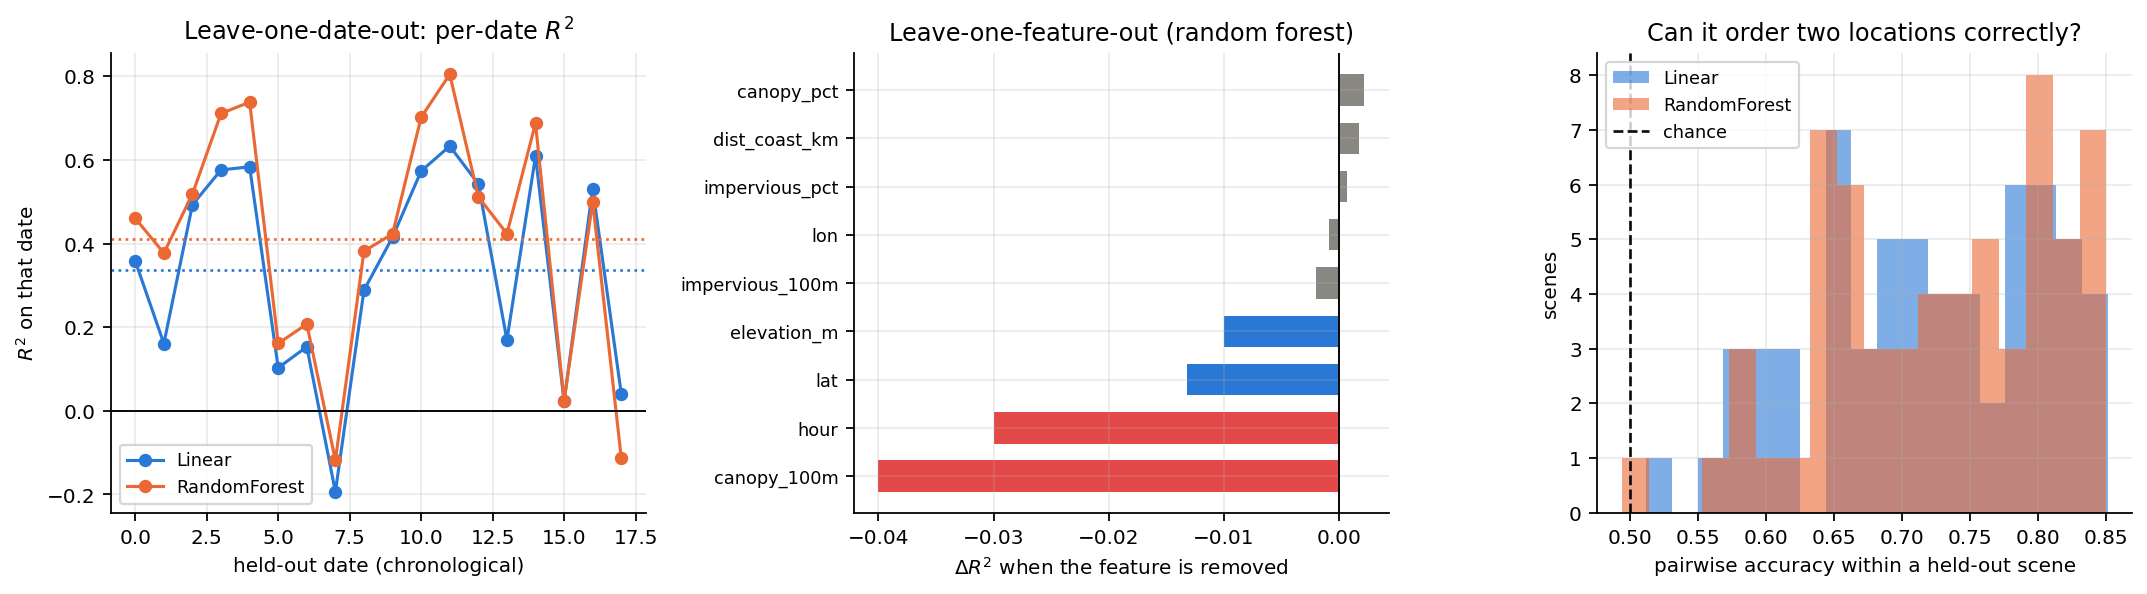
\includegraphics[width=\textwidth]{robustness.png}
\caption{Left: $R^2$ on each of the 18 held-out dates (dotted line: mean) --- the spread is
the point. Centre: change in $R^2$ when each feature is removed; three features score above
zero, meaning removal helps. Right: pairwise accuracy over 62 held-out scenes against the
\SI{50}{\percent} chance line.}
\label{fig:robust}
\end{figure}

\subsection{Results: route-level evaluation}
\label{sec:routes}
Model metrics do not tell us whether the system helps a walker. We sample
origin--destination pairs inside the LA box, rejecting any whose endpoints are not on
built-up land (impervious $> \SI{10}{\percent}$) or whose straight-line separation falls
outside \SIrange{0.8}{3}{\kilo\metre}, allocated evenly across three neighbourhood-canopy
strata (low/medium/high, \textbf{20 pairs per stratum}, 60
in total) so that leafy areas are represented rather than drowned out by the basin's
uniformly paved interior. A pair that turns out unroutable is discarded and replaced with a
fresh random draw \emph{from the same stratum} rather than simply dropped, so every stratum
reaches its target regardless of how many draws that takes; the low-canopy stratum needed
roughly 2{,}200 draws per 20 accepted pairs (a $\sim$\SI{1}{\percent} hit rate), since sparse
urban fringes often have no connected pedestrian graph at all. Each pair is scored at three
fixed local times (10:00, 13:00, 16:00) rather than at the system clock, and all routing
responses are cached so the sweeps below cost no further API calls. The result is
\textbf{60 pairs, 180 pair--hour evaluations}, with 2--7 distinct candidates each.

\paragraph{How much cooling is available at all?}
Before asking what the scorer does, we ask what it \emph{could} do: the predicted cooling of
the coolest eligible candidate relative to the shortest route. The median is
\SI{0.23}{\celsius}, the 90th percentile \SI{1.10}{\celsius}, the maximum
\SI{3.22}{\celsius}. Only \SI{14}{\percent} of pair--hours admit an alternative at least
\SI{1}{\celsius} cooler, \SI{32}{\percent} admit \SI{0.5}{\celsius}, and \SI{48}{\percent}
admit \SI{0.25}{\celsius}.

This is the central route-level result, and a sobering one: \textbf{for a short walk drawn
from our canopy-stratified sample, our method rarely finds a meaningfully cooler
alternative}. Cool
Routes reroutes over \SI{70}{\percent} of campus trips \citep{buo2026coolroutes}; we reroute
\SI{1.7}{\percent}. Three differences plausibly account for the gap, and only the first
concerns Los Angeles itself: \SI{70}{\metre} LST averages both sides of a street, so a
shaded-sidewalk detour is invisible to us by construction whereas \SI{1}{\metre} MRT resolves
it; a dense campus is not a random sample of a basin; and Cool Routes counts any cooler
alternative where we require \SI{1}{\celsius}. We read this as a statement about the
\emph{detection limit of coarse-resolution LST}, not as evidence that Los Angeles lacks
shaded detours.

\begin{table}[H]
\centering
\caption{Route evaluation, target setting $\tau = 1.3$ / minimum cooling \SI{1.0}{\celsius}.
``Available'' is what the best eligible candidate offered; the remaining columns describe
what was recommended, averaged over all evaluations including those where the shortest
route was kept. Lower blocks: by canopy stratum (60 pair--hours each), and the effect of the
minimum-cooling threshold at $\tau = 1.3$, pooled over all hours and strata.}
\label{tab:routes}
\small
\begin{tabular}{lrrrrrr}
\toprule
& Available (\si{\celsius}) & Cooling (\si{\celsius}) & Peak (\si{\celsius}) &
Canopy gain (pp) & Detour (\%) & Changed (\%) \\
\midrule
\multicolumn{7}{l}{\emph{By time of day}} \\
10:00 & 0.31 & 0.000 & 0.000 & $+0.00$ & 0.00 & 0.0 \\
13:00 & 0.52 & 0.040 & 0.033 & $+0.17$ & 0.24 & 3.3 \\
16:00 & 0.50 & 0.018 & 0.018 & $+0.13$ & 0.00 & 1.7 \\
\midrule
\multicolumn{7}{l}{\emph{By canopy stratum}} \\
Low (1.6\%)   & 0.28 & 0.000 & 0.000 & $+0.00$ & 0.00 & 0.0 \\
Mid (10.8\%)  & 0.43 & 0.018 & 0.012 & $+0.03$ & 0.24 & 1.7 \\
High (24.6\%) & 0.62 & 0.040 & 0.039 & $+0.27$ & 0.00 & 3.3 \\
\midrule
\multicolumn{7}{l}{\emph{Minimum-cooling threshold (\si{\celsius}), all hours and strata pooled}} \\
0.00 & --- & 0.125 & --- & --- & 5.92 & 43.9 \\
0.25 & --- & 0.107 & --- & --- & 3.07 & 18.3 \\
0.50 & --- & 0.082 & --- & --- & 2.14 & 11.1 \\
1.00 & --- & 0.019 & --- & --- & 0.08 & 1.7 \\
\bottomrule
\end{tabular}
\end{table}

Both available and realised cooling grow from morning to late afternoon, as expected once
solar load has accumulated, though the jump from 10:00 to 13:00 is sharper than the one from
13:00 to 16:00. The canopy-stratum block shows the gradient we built the sampler to find: the
high-canopy stratum offers more than double the available cooling of the low-canopy stratum
(\SI{0.62}{\celsius} against \SI{0.28}{\celsius}) and is rerouted roughly three times as
often. The threshold block confirms what we found earlier at a smaller sample: the
\emph{threshold}, not the weights, decides how interventionist the system is --- relaxing it
to \SI{0.25}{\celsius} raises the intervention rate from \SI{1.7}{\percent} to
\SI{18}{\percent} for a \SI{3.1}{\percent} mean detour, whereas sweeping the weights
(Figure~\ref{fig:tradeoff}) barely moves anything, because once the cap and threshold have
filtered the candidates there is usually only one survivor to choose between.

\begin{figure}[H]
\centering
\begin{subfigure}{0.46\textwidth}
  \centering
  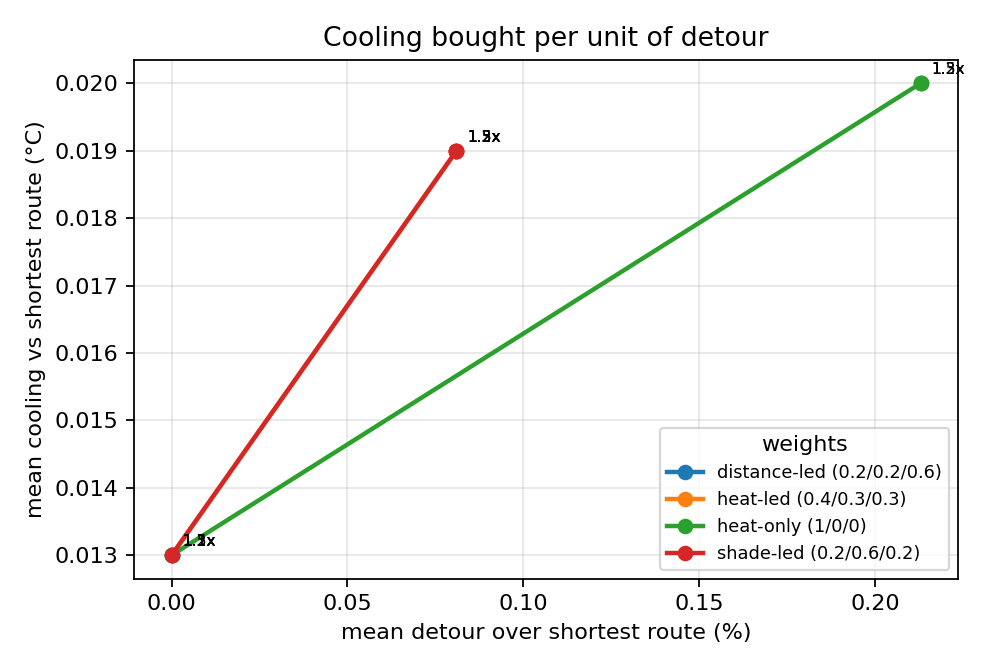
\includegraphics[width=\textwidth]{tradeoff.png}
  \caption{Cooling per unit of detour.}
  \label{fig:tradeoff}
\end{subfigure}\hfill
\begin{subfigure}{0.52\textwidth}
  \centering
  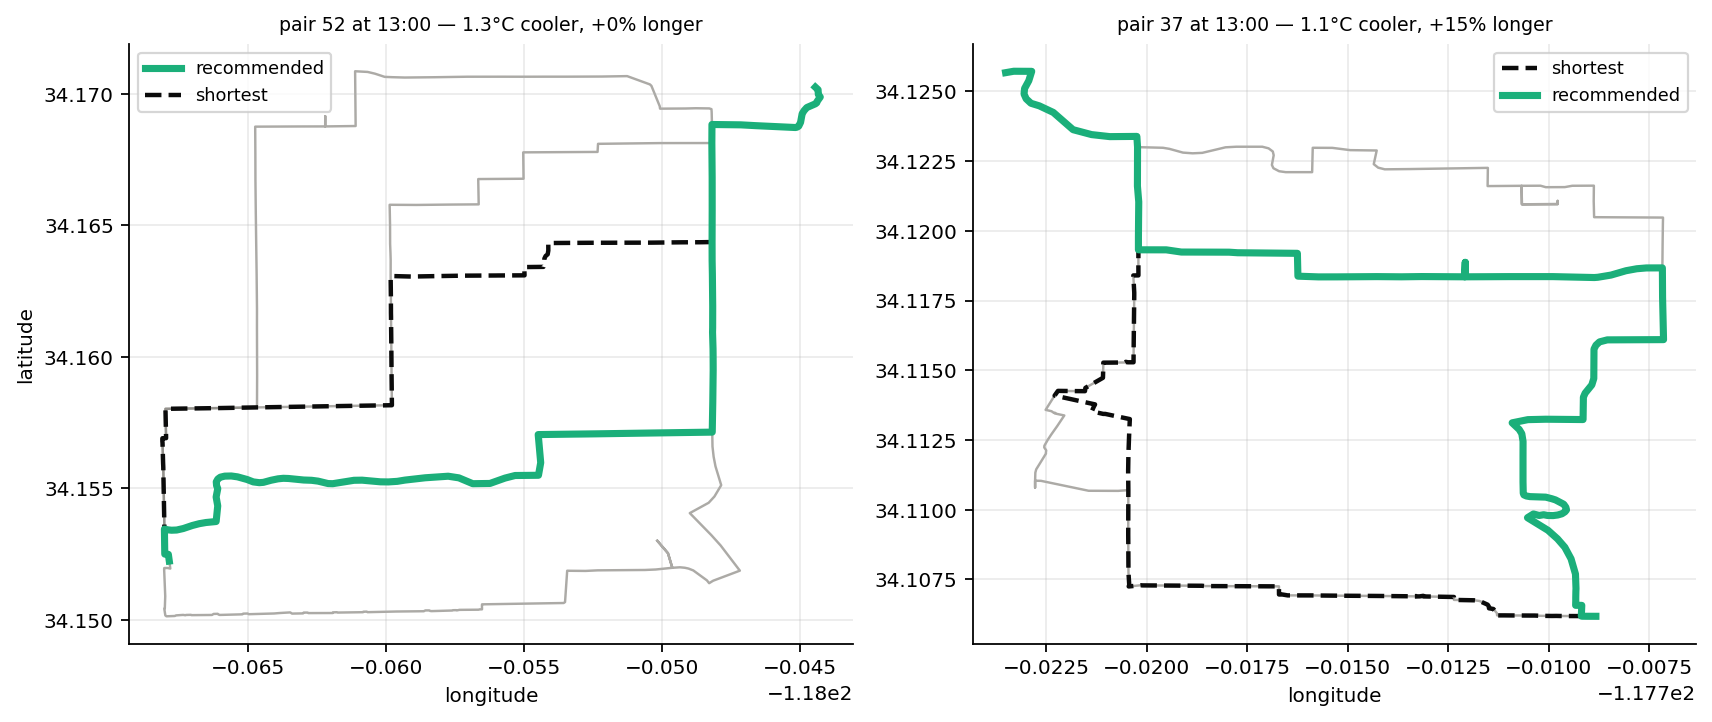
\includegraphics[width=\textwidth]{route_examples.png}
  \caption{Two pairs where the recommendation differs.}
\end{subfigure}
\caption{Route-level behaviour. Left: mean cooling against mean detour for four weightings
and four detour caps (annotated); the weightings are nearly indistinguishable, only the cap
and threshold move the outcome. Right: shortest (dashed) versus recommended (solid) path for
two pairs where the recommendation changed --- one at no distance cost at all, one trading
\SI{15}{\percent} extra distance for \SI{1.1}{\celsius}.}
\end{figure}

\paragraph{Caveats.}
These are \emph{predicted} differences from a model whose strict-split anomaly RMSE
(\SI{3.62}{\celsius}) exceeds almost every cooling margin in Table~\ref{tab:routes}; the
defensible claim is that the system \emph{ranks} candidates, which
Section~\ref{sec:robust-results} supports at \SI{72.7}{\percent} pairwise accuracy, not that
the per-route degree values are accurate. The canopy stratification also means this is not a
worst-case estimate: even the high-canopy stratum, sampled to be the most favourable case,
still changes only \SI{3.3}{\percent} of pair--hours (Table~\ref{tab:routes}), so stratifying
away from a uniform draw made the headline number more defensible, not less. We also tested,
and rolled back, a building-shadow
feature meant to probe the detection-limit argument directly: a neighbourhood-mean
sun-exposure covariate built from \num{2.3}~million LA County building footprints
\citep{lacounty2023lariac} was a net negative in the LST model (strict-split $R^2$
\num{0.343} with it against \num{0.348} without), and showed no clean separation between a
shade-aware and an LST-only route scorer at the sample sizes affordable here. We read this as
consistent with --- not a refutation of --- the detection-limit argument: \SI{70}{\metre} LST
and a neighbourhood-mean shadow feature share the same blind spot, sidewalk-scale shade, so
neither can confirm or deny it from this data. Resolving that needs the per-point shadow
signal used directly as routing cost, listed in Section~\ref{sec:remaining}.

%====================================================================
\section{Remaining Parts}
\label{sec:remaining}

\paragraph{Decisive: per-point shadow, not a neighbourhood average.}
Section~\ref{sec:routes} reports that a \emph{neighbourhood-mean} shadow covariate did not
help. That is a narrower result than it may look: averaging sun exposure over a
\SI{100}{\metre} window is exactly the operation that would erase a sidewalk-scale shadow
signal if one existed, since it mixes the shaded side of a street with the sunlit one. The
untested version of the detection-limit argument is a \emph{per-point} shadow cost --- solar
position against building footprints and heights, evaluated along the route itself and used
directly as routing cost rather than folded into the temperature model --- re-run to see
whether the reroute rate moves toward the \SI{70}{\percent} reported for campus-scale MRT
systems \citep{buo2026coolroutes}. This is our highest-priority experiment.

\paragraph{Decisive: validation against what a pedestrian feels.}
Section~\ref{sec:robust-results} validates the model against the \emph{satellite} --- it
predicts ECOSTRESS anomalies on unseen scenes --- but ECOSTRESS measures ground temperature,
not the air a person walks through, and certainly not thermal comfort. Nothing here closes
that gap. We plan to compare predicted anomalies against weather-station and crowd-sourced
air temperature; \citet{buo2026coolroutes} validated against a mobile
human-biometeorological platform, which is the standard to aim for.

\paragraph{Strengthening the evidence.}
Our 18 dates are why the leave-one-date-out interval is wide; we will extend the
download to May and September and, for the final report, train on one contiguous period and
test on a later one --- a better analogue of deployment than leave-one-date-out. Separately,
neither ECOSTRESS at \SI{70}{\metre} nor NLCD at \SI{30}{\metre} can separate the two sides
of a street, so a higher-resolution canopy product would let recommendations operate at the
scale a pedestrian experiences.

\paragraph{Extensions.}
An \textbf{equity analysis} --- canopy in Los Angeles is unevenly distributed
\citep{hoffman2020redlining}, so the \emph{availability} of a cooler route likely is too, and
we want to know whether the system helps least where help is needed most. A \textbf{human
evaluation} in which participants walk both routes and report perceived comfort.
\textbf{Night-time routing}, which the system currently declines (returning the shortest
path outside 8--19\,h) because lighting and perceived safety, not heat, govern that regime.

%====================================================================
\section*{Team Member Roles}
\small
\begin{tabular}{@{}p{0.22\textwidth}p{0.74\textwidth}@{}}
\toprule
\textbf{Ethan Chiu} & TODO: describe contribution (e.g.\ ECOSTRESS acquisition and quality
filtering; data funnel analysis). \\
\textbf{Junseo Lee} & TODO: describe contribution (e.g.\ modelling pipeline, evaluation-split
design, robustness experiments). \\
\textbf{Nathan Nguyen} & TODO: describe contribution (e.g.\ routing integration, route-level
evaluation, demo application). \\
\textbf{Sinchana Nama} & TODO: describe contribution (e.g.\ land-cover processing, derived
features, exploratory analysis and figures). \\
\bottomrule
\end{tabular}
\normalsize

\medskip
\noindent All four members contributed to the problem formulation, the literature review and
the writing of this report.

%====================================================================
\section*{Reproducibility}
All results in this report are produced by scripts in the project repository:
\texttt{clip\_rasters.py} (raster preparation), \texttt{build\_features.py} (derived rasters),
\texttt{build\_dataset.py} (data fusion, Table~\ref{tab:funnel}), \texttt{train.py} (shipped
model), \texttt{experiments.py} (Tables~\ref{tab:features} and~\ref{tab:models}),
\texttt{robustness.py} (Section~\ref{sec:robust-results}), \texttt{evaluate\_routes.py}
(Section~\ref{sec:routes}) and \texttt{make\_figures.py} (all figures). Random seeds are
fixed in \texttt{config.yaml}, which also holds every filter threshold, feature list and
scoring weight used above. The building-shadow ablation reported as a caveat in
Section~\ref{sec:routes} is the one exception: it was implemented, measured, found to not
help, and removed from the shipped pipeline, so the exact numbers quoted are not
re-runnable from the current script set.

\bibliographystyle{plainnat}
\bibliography{references}

\end{document}
